\subsection{Why virtualized HPC?}
Although HPC workloads are most often run on bare-metal systems, this has started to change 
with the realization that many of the benefits that virtualization offers to enterprises 
can often also add value in HPC environments. The following are among those benefits:
\begin{itemize}
	\item Supports a more diverse end-user population with differing software requirements
	\item Provides multi-tenancy data security by isolating user workloads into separate VMs
	\item Provides fault isolation, root access, and other capabilities not available in traditional HPC environments
	\item Creates a more dynamic execution environment in which VMs and their encapsulated workloads 
	can be live-migrated across the cluster for load balancing, for maintenance, for fault avoidance, and so on
\end{itemize}

In addition to above benefits, the performance of HPC applications on virtual platform has dramatically 
improved over the past years. This is especially true for HPC throughput workloads, which in contrast to MPI workloads, 
consist of a large number of independent tasks that can be executed in parallel. Throughput workloads represent a 
significant portion of HPC workloads and include life sciences, electronic design automation, image rendering, etc. 
Studies have demonstrated that the performance gap between virtual and bare metal for HPC throughput workloads is 
closing, with just 1 or 2 percentage difference~\cite{michael2018overcommit}. 
%as shown in Figure \ref{fig:perf_gap}~\cite{michael2018overcommit}.

% \begin{figure}[!t]
%    \begin{center}
%        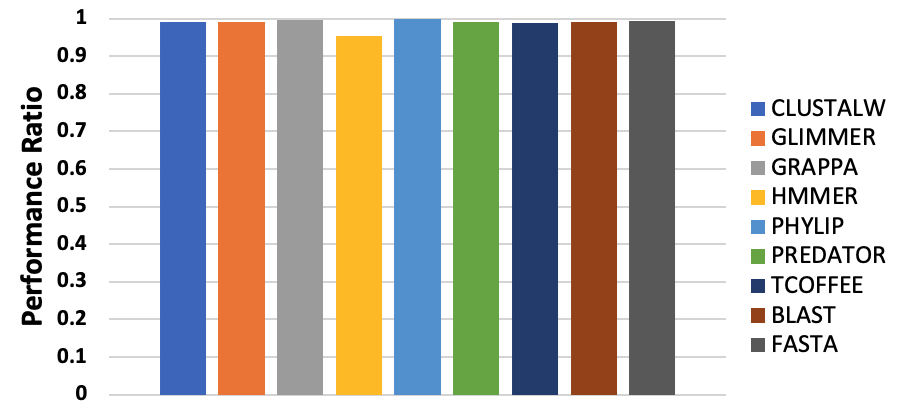
\includegraphics[width=\columnwidth]{Figures/perf_gap}
%    \end{center}
%    \caption{Performance ratio between virtual and bare metal for a set of life sciences workloads 
%    from BioPerf benchmark suite~\cite{1526013}. Higher is better. VMware ESXi 5.5 is used as the hypervisor.}
%    \label{fig:perf_gap}
%  \end{figure}

\subsection{HPC cloud resource allocation}
Virtualization brings new flexibility to HPC. With that flexibility, however, one must be careful to configure 
the cloud environment to simultaneously achieve both agility and high performance.
Although it is possible to create a single virtual cluster that spans an entire data center partition
with one maximally sized VM per node, this approach misses the opportunity to enable several important 
virtualization benefits. Among these are the ability to support per-tenant or per-project software stacks as well 
as security and fault separation between the tenant workloads. In the more typical case, multiple virtual 
clusters should be hosted simultaneously on the physical cluster for isolation between tenants.

In a situation in which a tenant is using resources intensively, it might make most sense to assign 
a dedicated subset of hardware to the tenant and to configure VMs on those nodes appropriately. 
With two such tenants, one can either place their VMs on a non-overlapping set of nodes (Figure~\ref{fig:allocation1})
or place them on the same nodes, being careful to size their VMs to avoid any over-commitment (Figure~\ref{fig:allocation2}). 
%Typically, the size of each such VM is set to the number of cores available in each underlying physical CPU to take 
%advantage of the hardware NUMA topology. 
%This approach works well if the VMs are so heavily loaded that 
%few cycles are left unused on each node. However, it is often the case that such projects do not in actuality 
%show this degree of resource intensity. Although they might be very busy and resource constrained in some 
%time periods, they can also be less busy and even idle in other periods. In such cases, sizing VMs as 
%described--so that they partition the available physical cores--can lead to commensurate losses in 
%throughput because the idle CPUs serving one VM are not available to the other busy VM.
The major flaw with these approaches is that resources are statically partitioned and thus liable to under-utilization. 
Although tenants might be very busy in some 
time periods, they can also be less busy and even idle in other periods. In such cases, sizing VMs as 
described above can lead to commensurate losses in 
throughput because the idle resources serving one VM are not available to the other busy VM.

\begin{figure}
     \centering
     \begin{subfigure}[b]{0.45\textwidth}
         \centering
         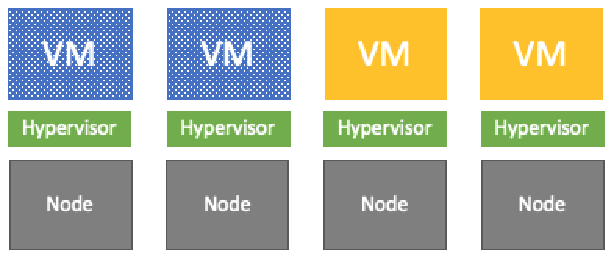
\includegraphics[width=\textwidth]{Figures/allocation1}
         \caption{Partition on non-overlapping nodes}
         \label{fig:allocation1}
     \end{subfigure}
     \hfill
     \begin{subfigure}[b]{0.45\textwidth}
         \centering
         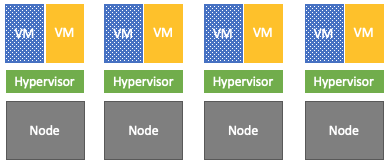
\includegraphics[width=\textwidth]{Figures/allocation2}
         \caption{Partition on same nodes}
         \label{fig:allocation2}
     \end{subfigure}
     \caption{Example of traditional static allocation with four hosts and two tenants. Gray VMs for one tenant and yellow VMs for the other.}
     \label{fig:static_allo}
\end{figure}

\subsection{Resource over-commitment}
The key to avoiding the above resource waste issue is resource over-commitment. In a 
virtualized environment, resource over-commitment means configuring VMs with more than the available 
physical resources. For example, on a host with 4 CPU cores and 8 GB memory, one could create and power on two VMs each 
with 4 virtual CPUs and 6 GB virtual memory. Resource over-commitment has been studied, but previous works did not optimize for HPC workloads 
and only considered CPU over-commitment~\cite{tran2019,Tesfatsion2018}.

CPU over-commitment is accommodated by multiplexing virtual 
CPUs onto the physical CPU cores. In a modern hypervisor like VMware ESXi, a share-based mechanism can be enabled  
in the scheduler so that each VM can get a different portion of the physical CPUs based on its configured shares, 
even in the case of over-commitment~\cite{vmware2013scheduler}. Furthermore, a work-conserving scheduler 
allows one VM to consume more than its fair CPU share if there are idle cycles from other VM(s). 
Memory over-commitment, on the other hand, is more challenging since multiplexing is not 
applicable. It is achieved by a set of memory reclamation techniques, including transparent page sharing (TPS), 
ballooning, compression, and hypervisor swapping~\cite{Waldspurger:2002:MRM:844128.844146,banerjee2013memory}. These techniques differ in the incurred 
overhead and are individually controlled by the hypervisor based on system memory state.  

